\lstinputlisting[language=bash,basicstyle=\small]{python_codes/fieldstone_78/keywords}

\begin{center}
Code at \url{https://github.com/cedrict/fieldstone/tree/master/python_codes/fieldstone_78}
\end{center}

\par\noindent\rule{\textwidth}{0.4pt}

%%%%%%%%%%%%%%%%%%%%%%%%%%%%%%%%%%%%%%%%%%%%%%%%%%%%%%%%%%%%%%%%%%%%%%%%%%%%%%%%%%%%%%%%%%%%%%%%%%%%


Although the $Q_1\times P_0$ is not LBB-stable (see Section~\ref{ss:LBBcond})
it has been proven that some spatial arrangements of this element can be, such as the
following macro-element:

\begin{center}
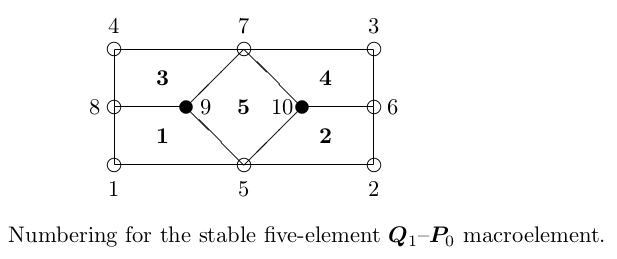
\includegraphics[width=5cm]{python_codes/fieldstone_78/images/elsw}
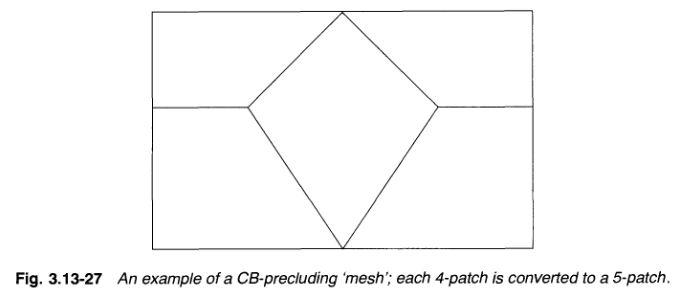
\includegraphics[width=5cm]{python_codes/fieldstone_78/images/grsa}\\
{\captionfont Left: Fig 3.12 of Elman et al book \cite{elsw}.
Right: Taken from Gresho \& Sani's book \cite{grsa}: "For fans of $Q_1Q_0$ who want 
guaranteed optimal convergence of both u and p (with however larger error 
constants caused by the distorted shapes?), one way to assure this is
to discretise via the macro elements above, each composed of five $Q_1Q_0$
quadrilaterals. Such checkerboard-killer meshes have been employed in practice
by (at least) Bath\'e \cite{chba93}. Both the macro-element and the proof are
due to Stenberg \cite{sten84}."}
\end{center}

\begin{center}
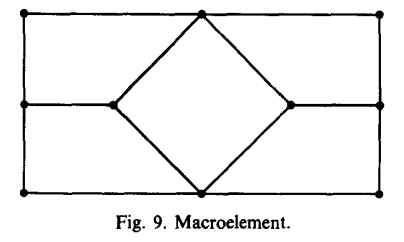
\includegraphics[width=5cm]{python_codes/fieldstone_78/images/chba93}\\
{\captionfont Taken from Chapelle \& Bathe \cite{chba93}: "the numerical inf-sup test is passed for this mesh and in fact,
this behavior was proven analytically (see Brezzi \& Fortin \cite{brfo}, see also Le Tallec \& Ruas \cite{leru86}).}
\end{center}

\begin{center}
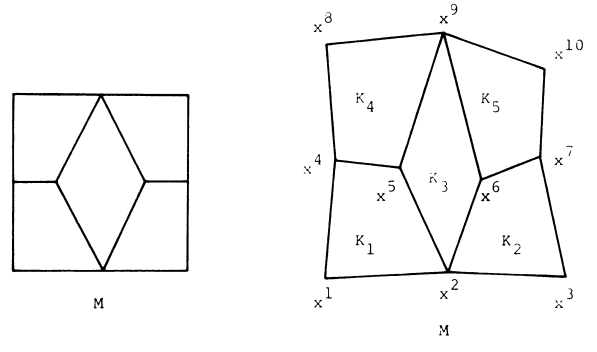
\includegraphics[width=5cm]{python_codes/fieldstone_78/images/sten84}
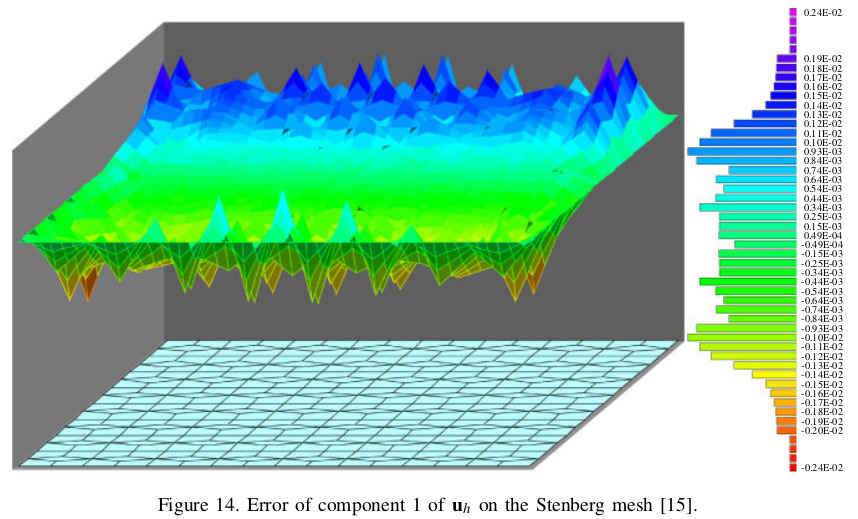
\includegraphics[width=5cm]{python_codes/fieldstone_78/images/qizh07}\\
{\captionfont Left: Taken from Stenberg (1984) \cite{sten84}. 
Right: Taken from Qin \& Zhang (2007) \cite{qizh07}.}
\end{center}

On the following a mesh is shown which consists of $16\times 16$ macroelements:

\begin{center}
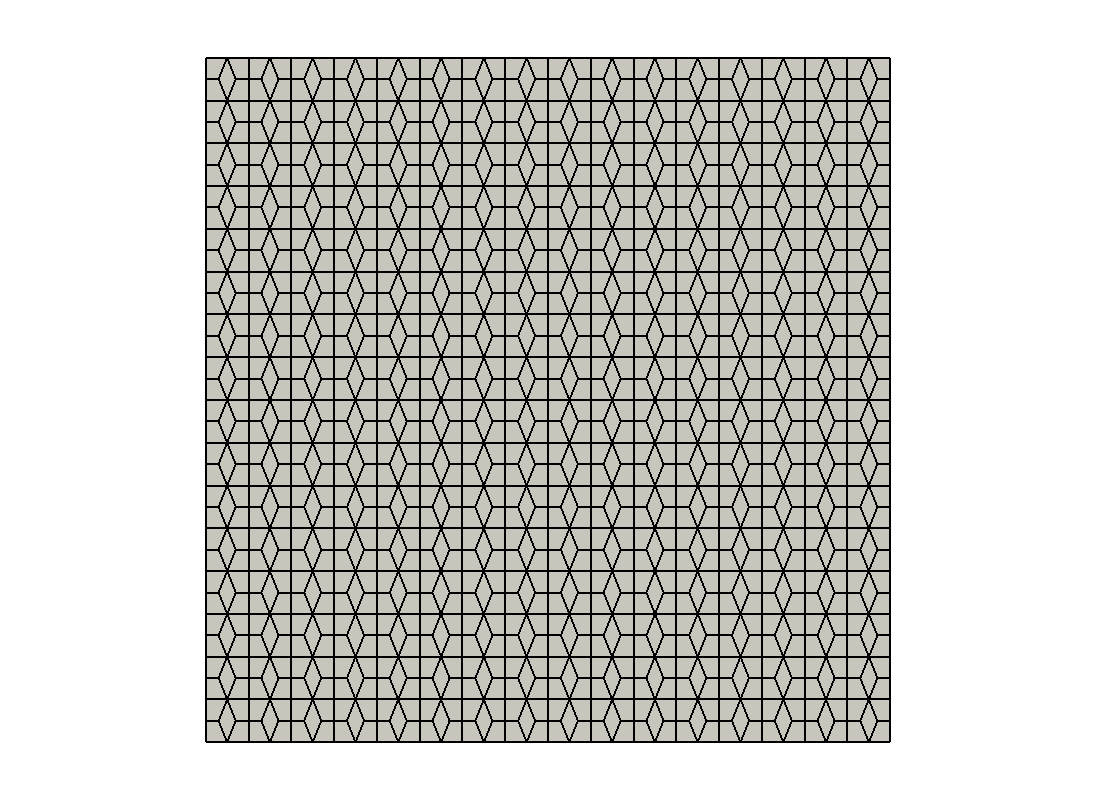
\includegraphics[width=8cm]{python_codes/fieldstone_78/images/mesh}\\
{\captionfont Mesh composed of 16x16 macroelements}
\end{center}
Note that in this implementation all 5 elements of the macro-element have the 
same area. 

Normalisation is achieved by setting $p=0$ on the last element and then 
renormalising the pressure field.

%........................
\paragraph{Results - mms}

We start with the Donea \& Huerta manufactured solution (see Section~\ref{mms1}) and 
proceed to compute the velocity and pressure error convergence as a function of the 
element size which is take to be $h = \sqrt{L_xL_y/nel}$. We see that 
the errors converge as expected, quadratically for the velocity and linearly for the pressure.
Rather interestingly the projection of the pressure onto the nodes has a convergence rate 
higher than the raw elemental pressure. 

\begin{center}
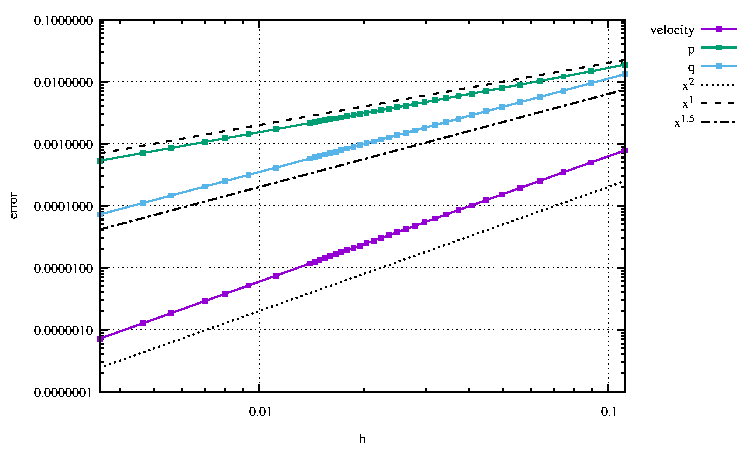
\includegraphics[width=7cm]{python_codes/fieldstone_78/results/mms/errors.pdf}
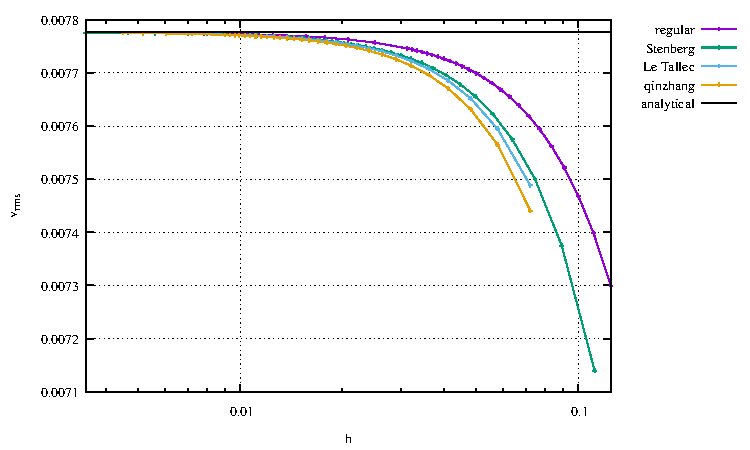
\includegraphics[width=7cm]{python_codes/fieldstone_78/results/mms/vrms.pdf}
\end{center}

On the following figures the pressure is plotted against the analytical solution and 
we see that there is no checkerboarding occurring:

\begin{center}
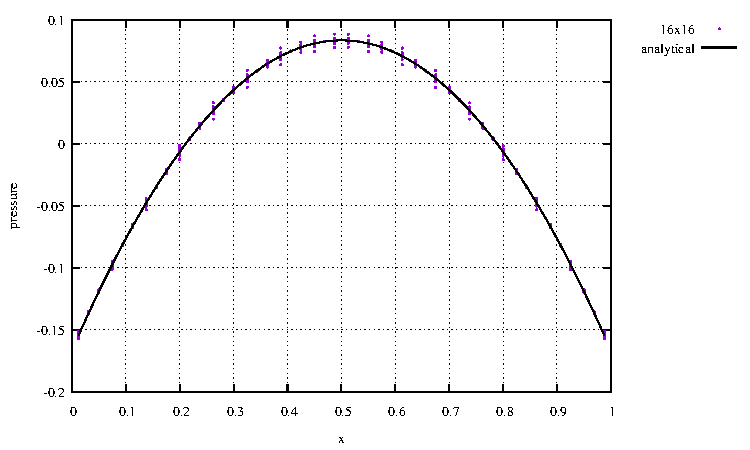
\includegraphics[width=5cm]{python_codes/fieldstone_78/results/mms/pressure16}
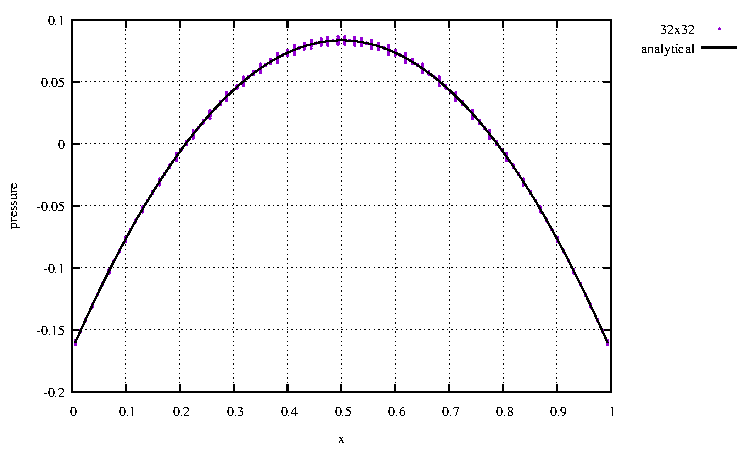
\includegraphics[width=5cm]{python_codes/fieldstone_78/results/mms/pressure32}
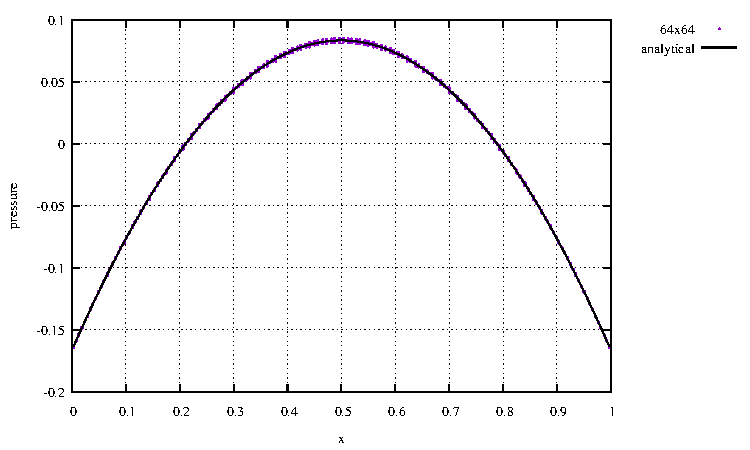
\includegraphics[width=5cm]{python_codes/fieldstone_78/results/mms/pressure64}\\
\end{center}

Rather interestingly the pressure error is the largest next to the boundaries:
\begin{center}
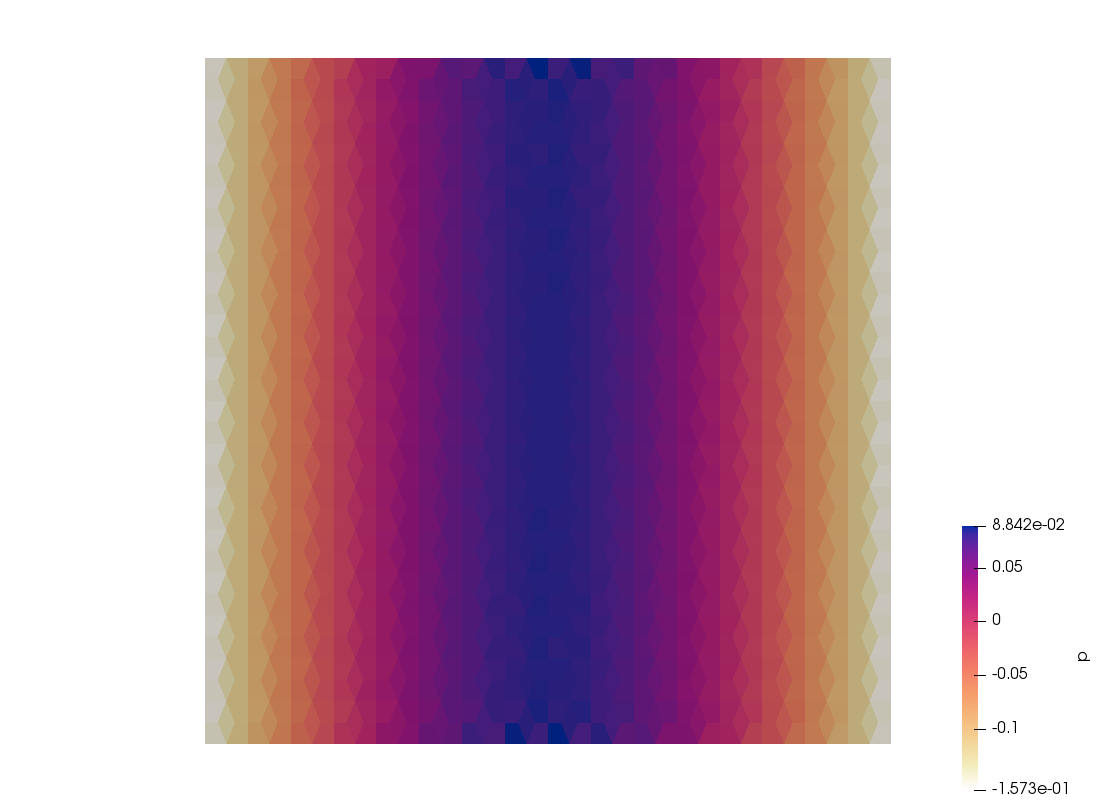
\includegraphics[width=7cm]{python_codes/fieldstone_78/results/mms/p16x16}
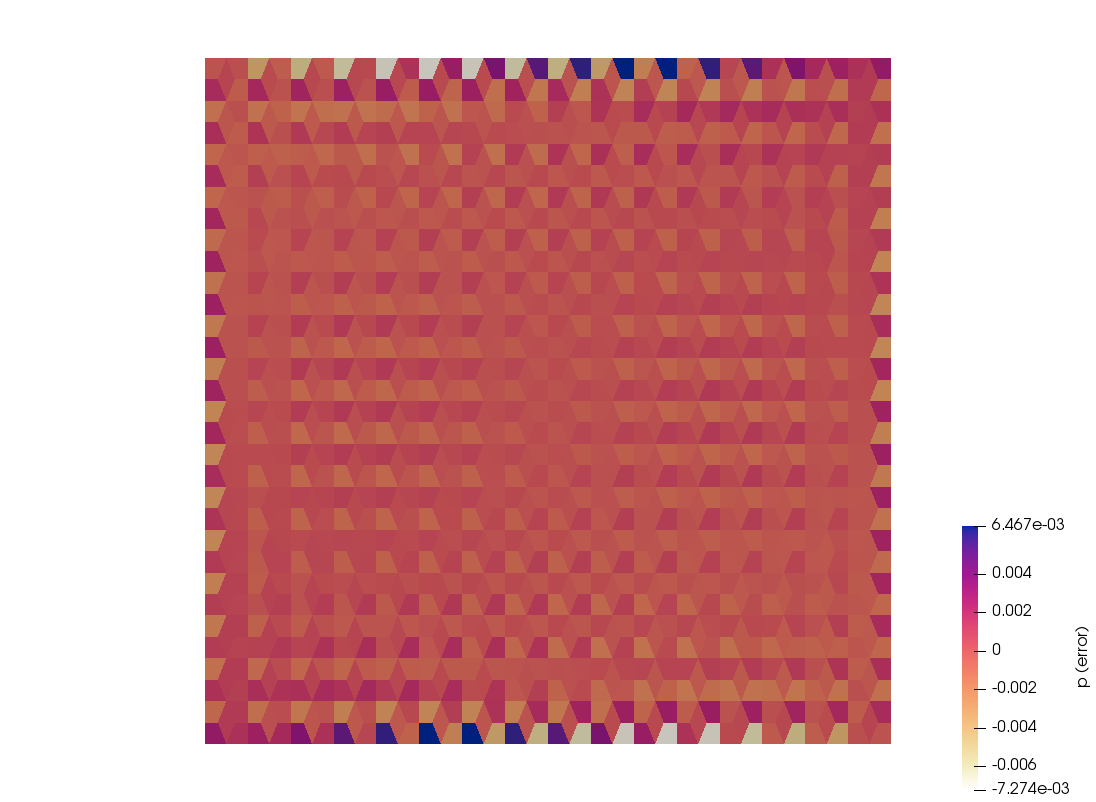
\includegraphics[width=7cm]{python_codes/fieldstone_78/results/mms/p16x16_error}\\
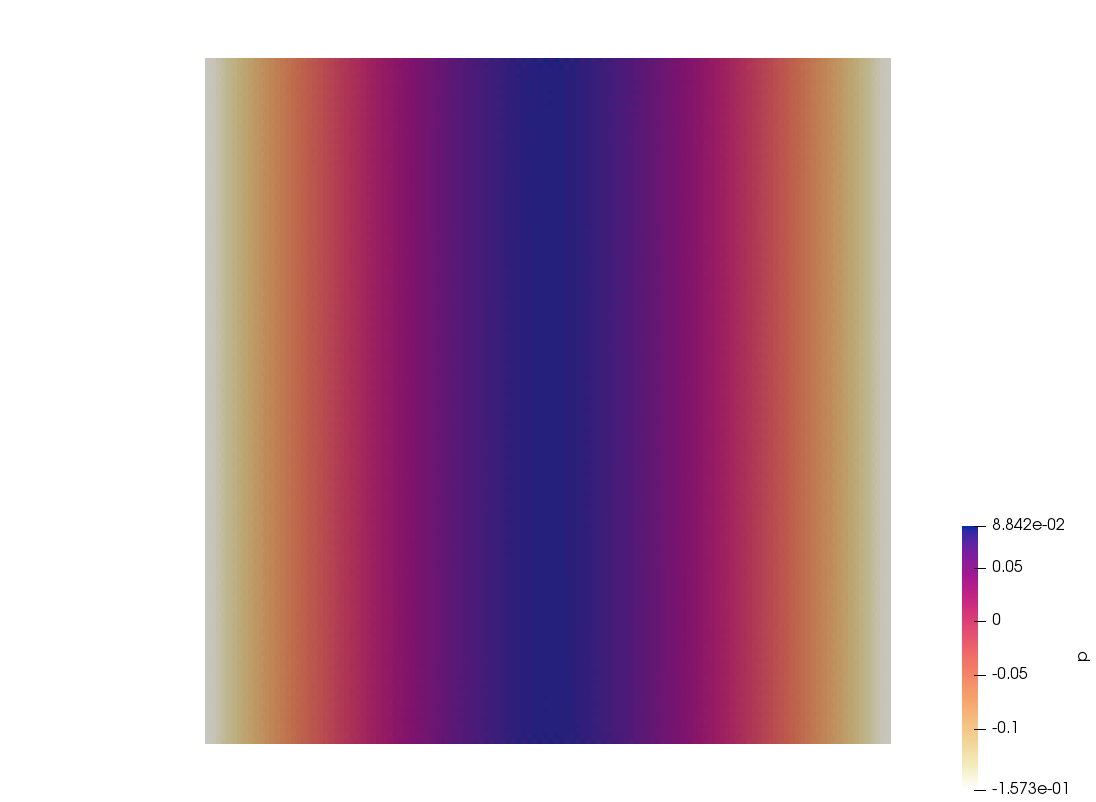
\includegraphics[width=7cm]{python_codes/fieldstone_78/results/mms/p64x64}
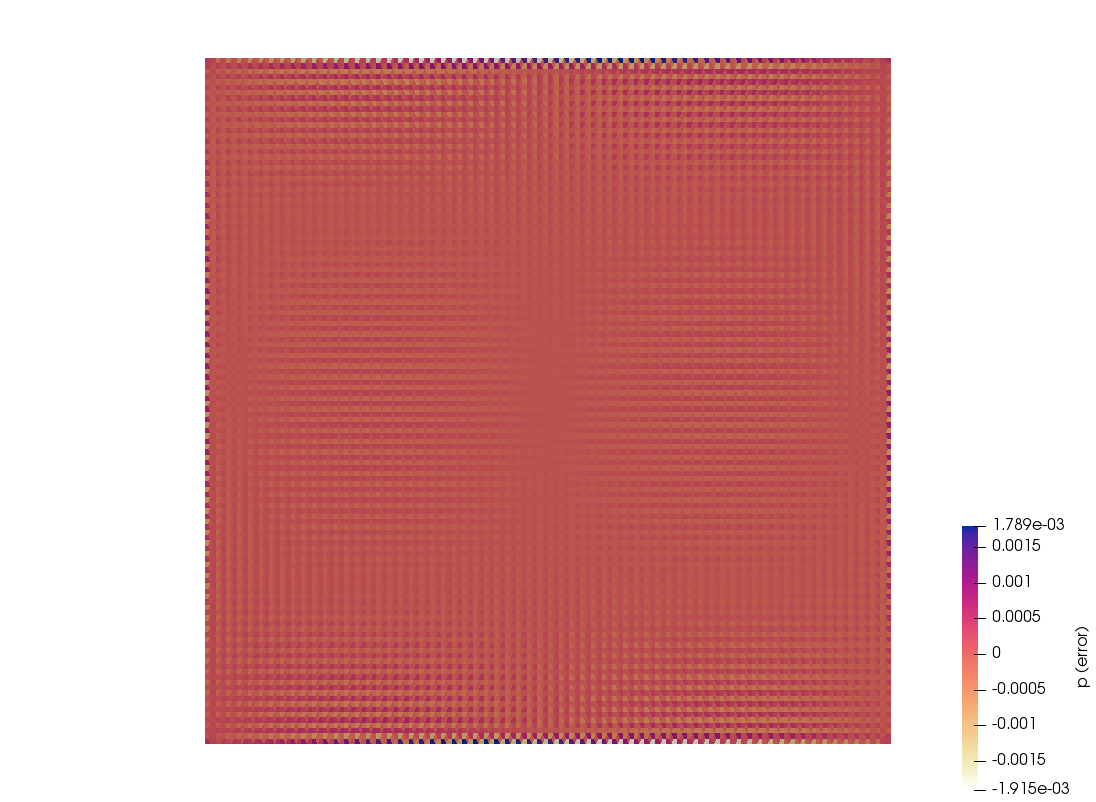
\includegraphics[width=7cm]{python_codes/fieldstone_78/results/mms/p64x64_error}\\
{\captionfont Top row: 16x16 mesh, bottom row: 64x64 mesh}
\end{center}

Discussion: what is the real advantage of such a macro-element? it is LBB stable, so 
iterative solver will work optimally, and the pressure has no checkerboard. 
Also the number of non-zeros per line of the matrix is small.  
On the other hand it is anisotropic since the 'diamonds are vertical'. 
Also if one would consider a macro-element as an element, it counts 10 velocity nodes and 5 pressures, 
which makes it much more expensive than a $Q_2\times Q_1$ element of the same size...

%..................................
\paragraph{Results - sinking block}

The block has size 0.25x0.25, centered in the domain. No-slip boundary conditions are imposed on all 
sides. The buoyancy force $\rho g_y$ is -1 in the block and zero elsewhere. Viscosity is constant and 
equal to 1 everywhere. 

\begin{center}
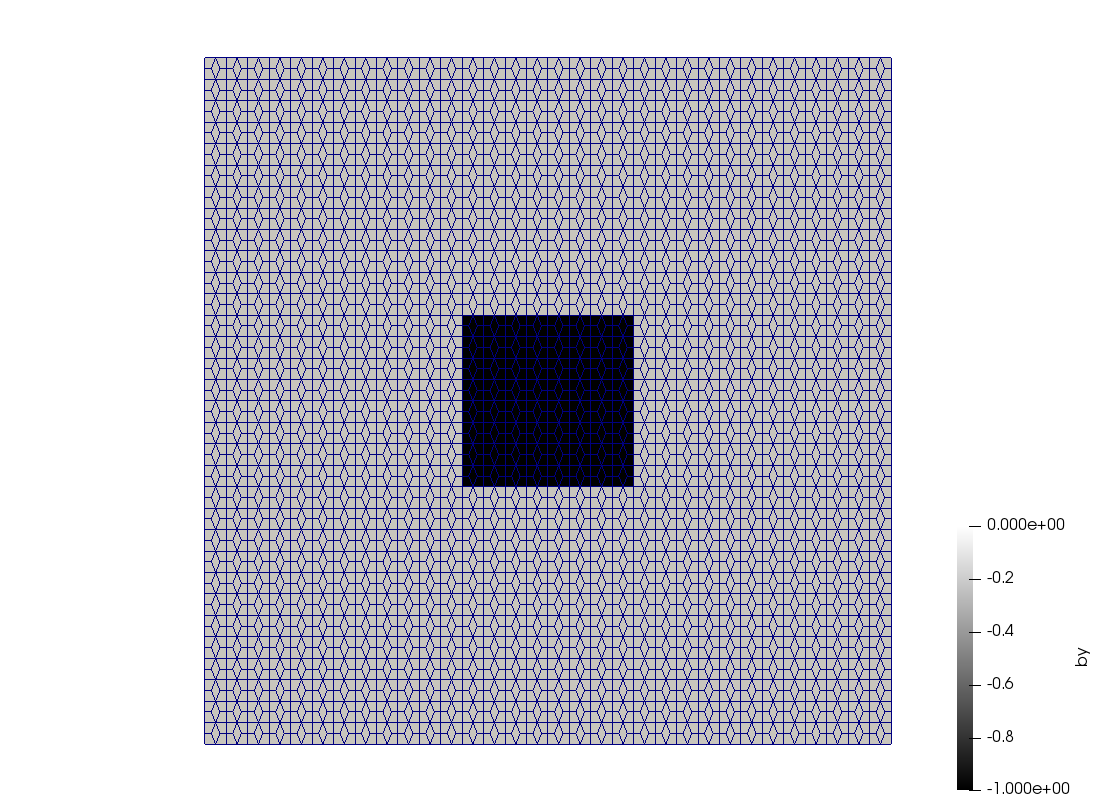
\includegraphics[width=7cm]{python_codes/fieldstone_78/results/block/by}
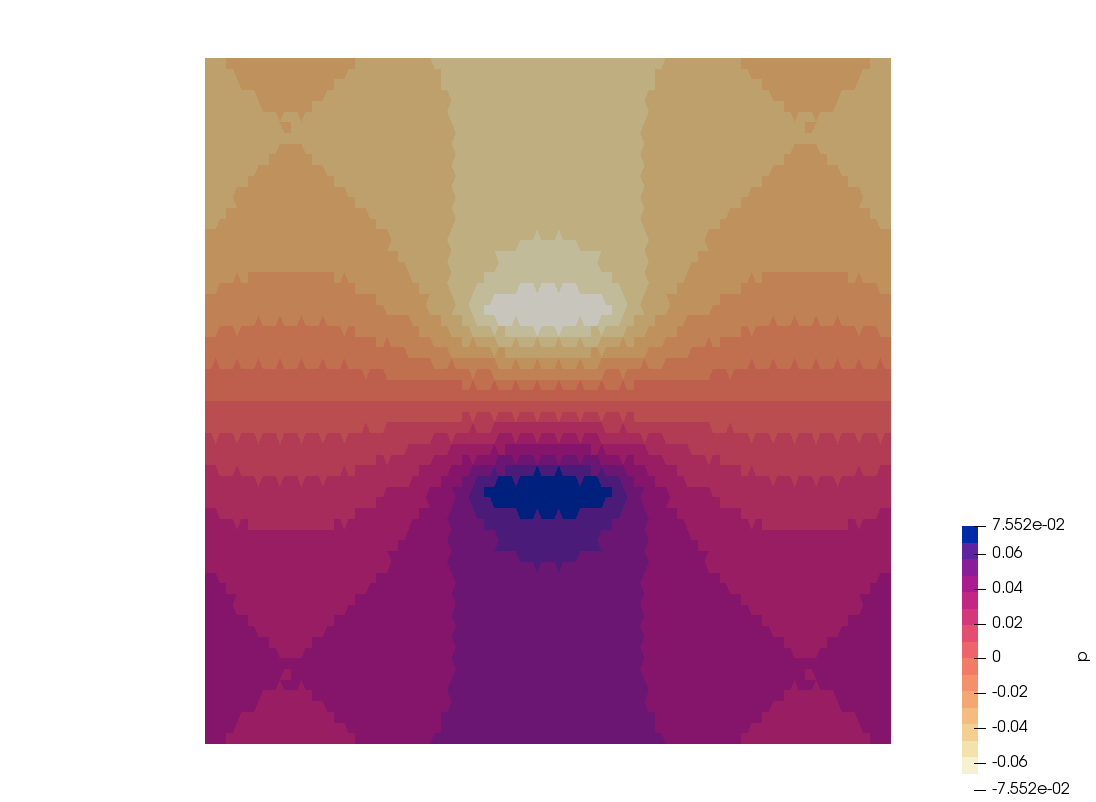
\includegraphics[width=7cm]{python_codes/fieldstone_78/results/block/p32}\\
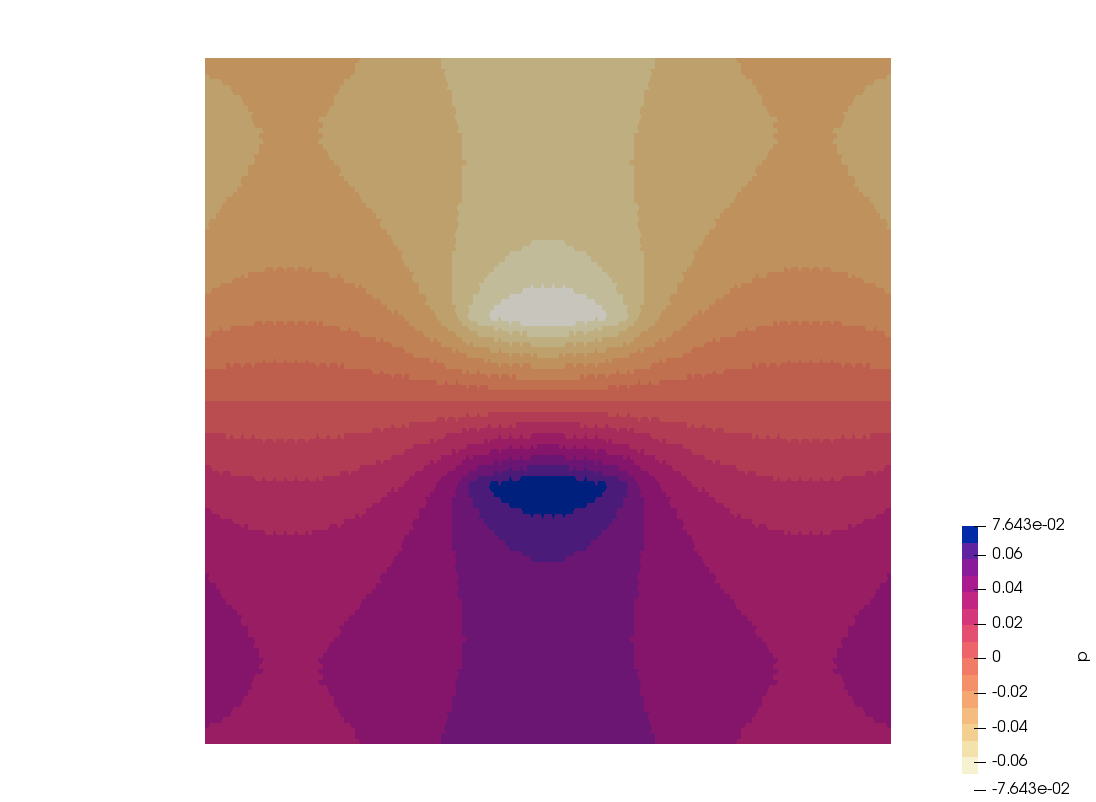
\includegraphics[width=7cm]{python_codes/fieldstone_78/results/block/p64}
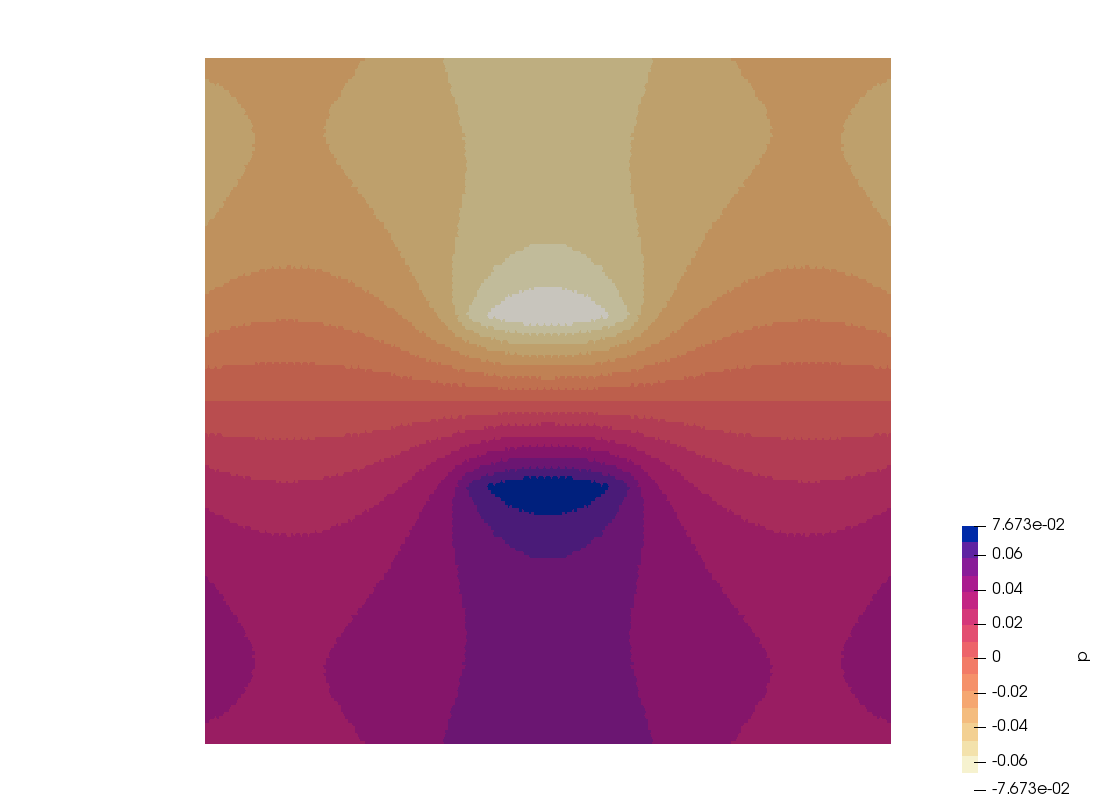
\includegraphics[width=7cm]{python_codes/fieldstone_78/results/block/p96}\\
{\captionfont buoyancy term $b_y$; pressure at resolutions 32x32, 64x64 and 96x96}
\end{center}

We then proceed with $\rho g_y=-1$ in the surrounding fluid and $\rho g_y=-1+\delta$ in the block.
The velocity and presure fields are shown in the following figure for various values of $\delta$.
We see that when the density of the block approaches the one of the surrounding fluid the 
velocity field shows abnormal stripes while the pressure field looks hydrostatic.   

\begin{center}
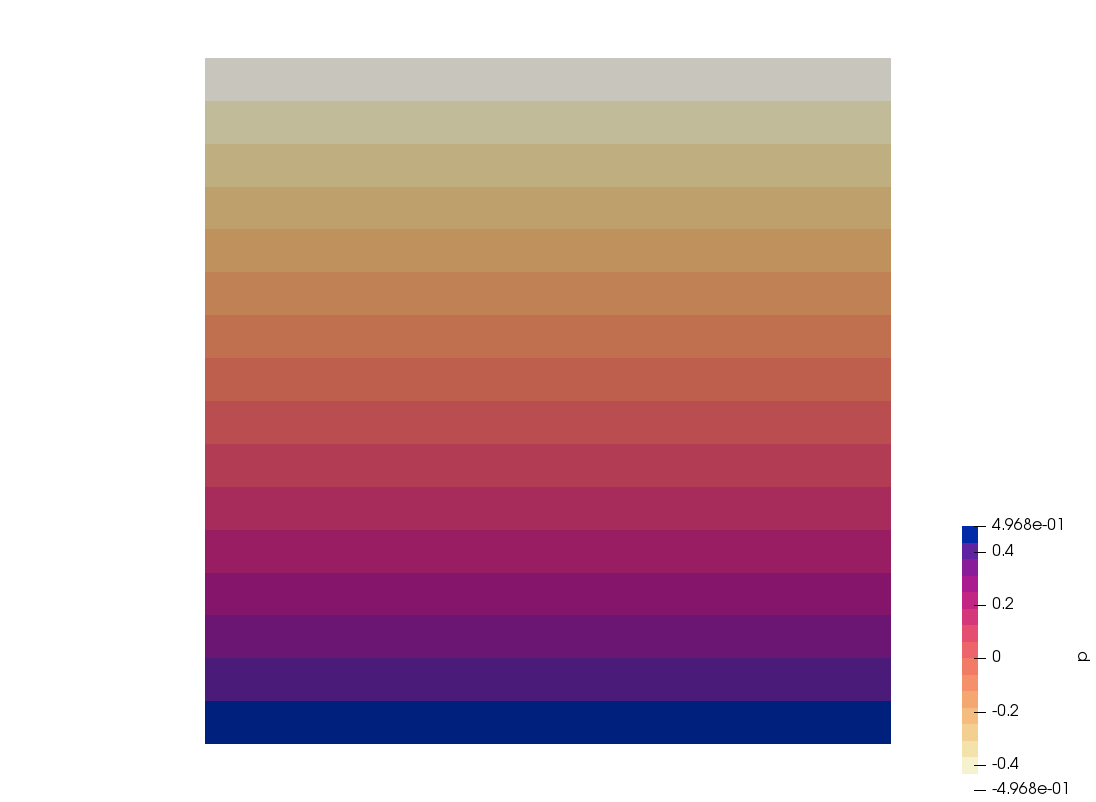
\includegraphics[width=3.84cm]{python_codes/fieldstone_78/results/block/p_delta0p001}
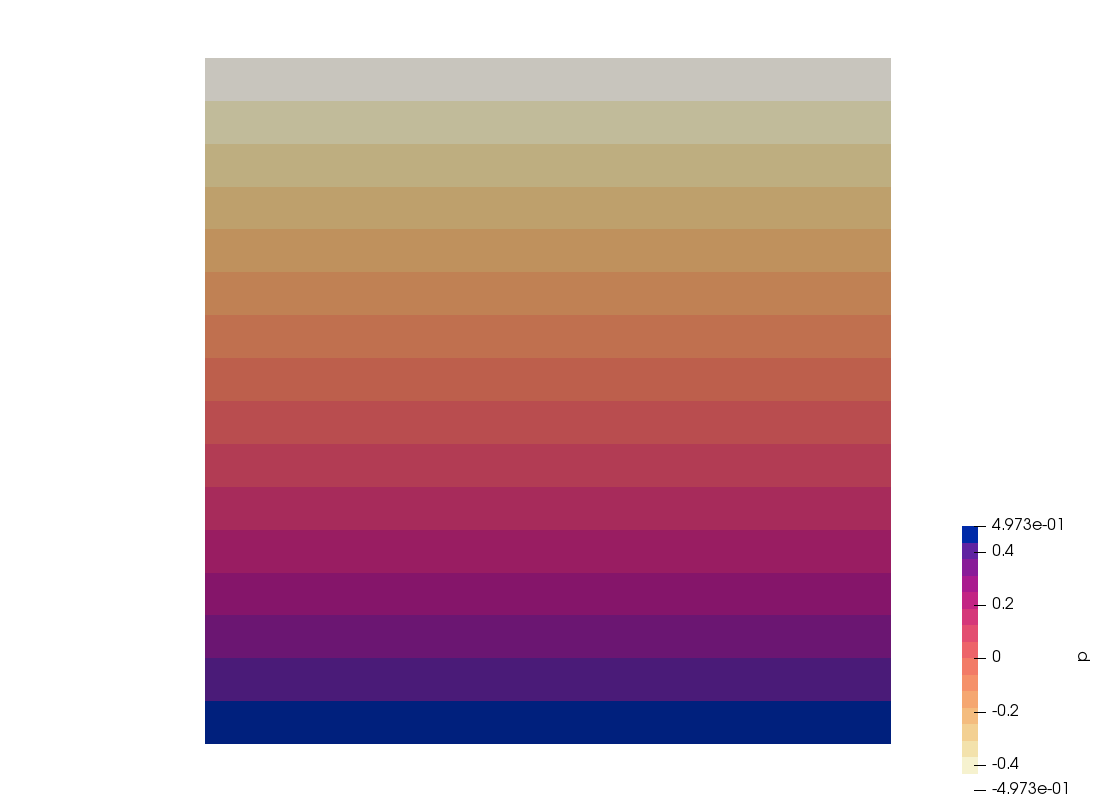
\includegraphics[width=3.84cm]{python_codes/fieldstone_78/results/block/p_delta0p01}
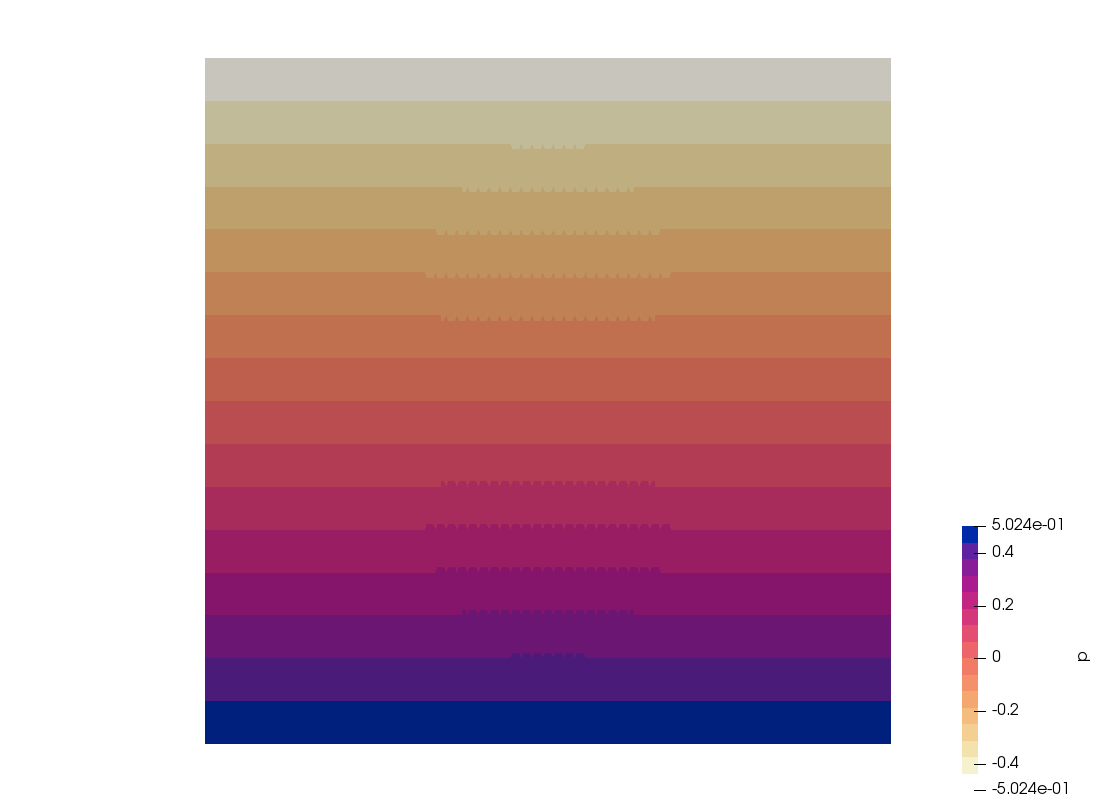
\includegraphics[width=3.84cm]{python_codes/fieldstone_78/results/block/p_delta0p1}
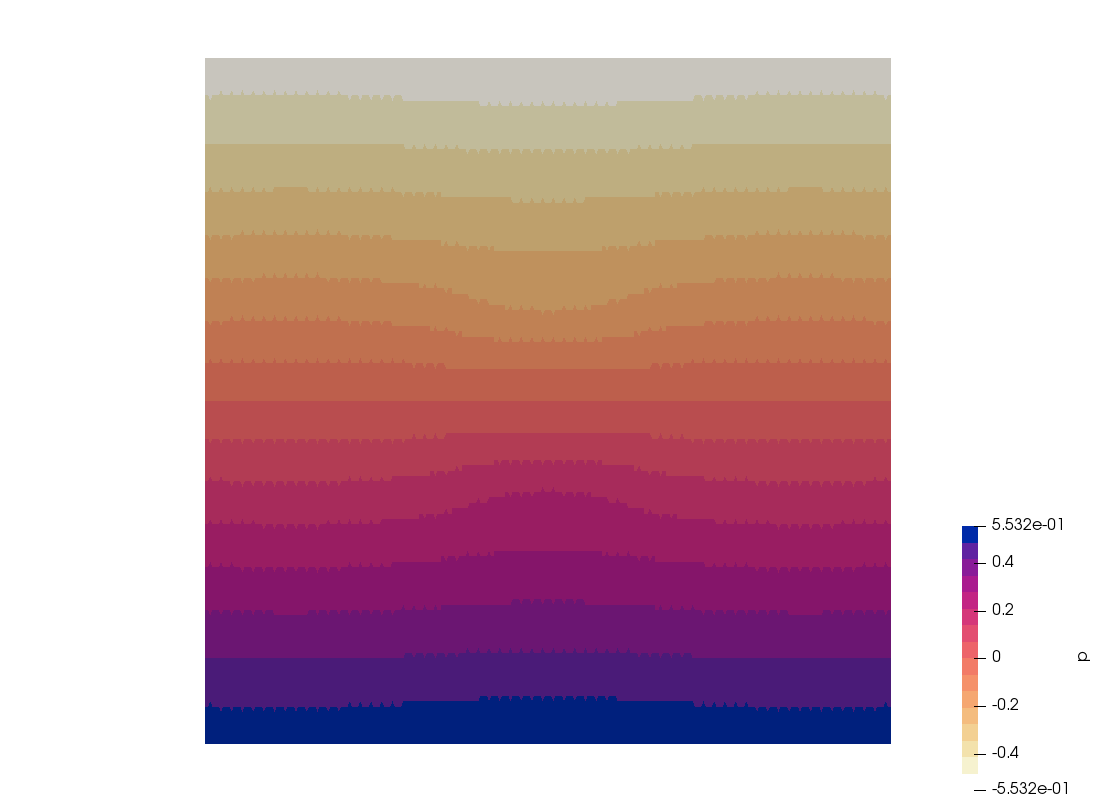
\includegraphics[width=3.84cm]{python_codes/fieldstone_78/results/block/p_delta1}\\
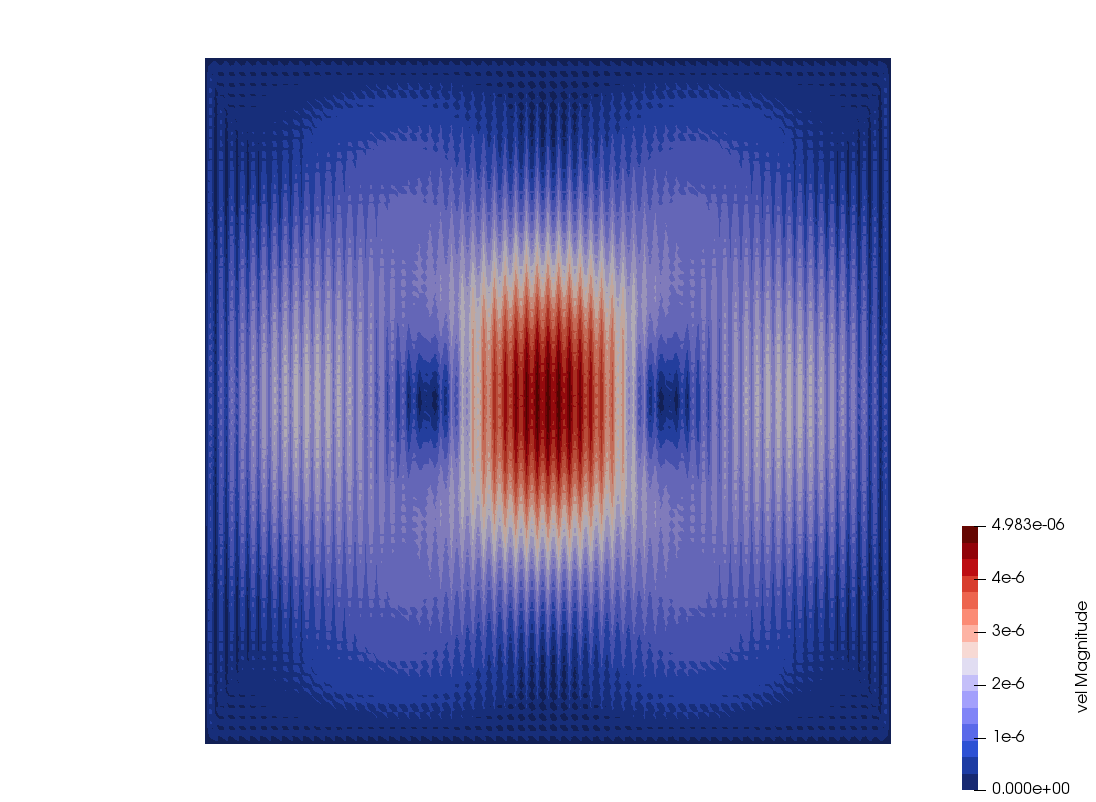
\includegraphics[width=3.84cm]{python_codes/fieldstone_78/results/block/vel_delta0p001}
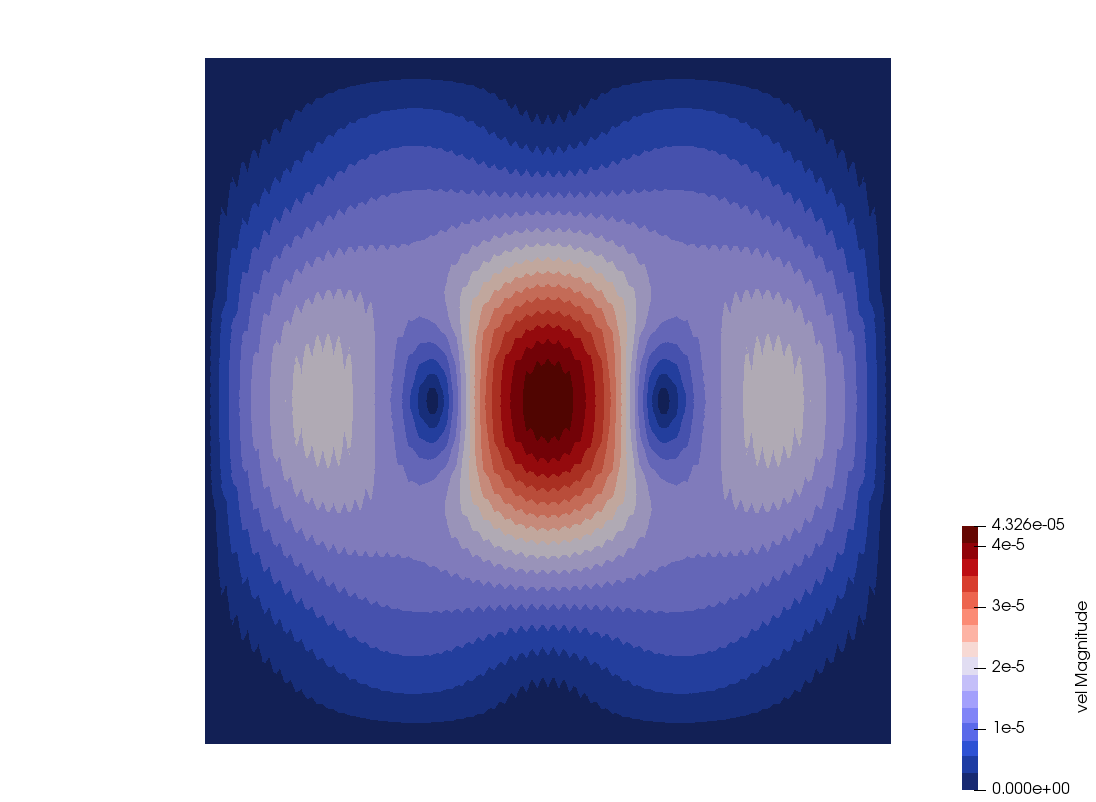
\includegraphics[width=3.84cm]{python_codes/fieldstone_78/results/block/vel_delta0p01}
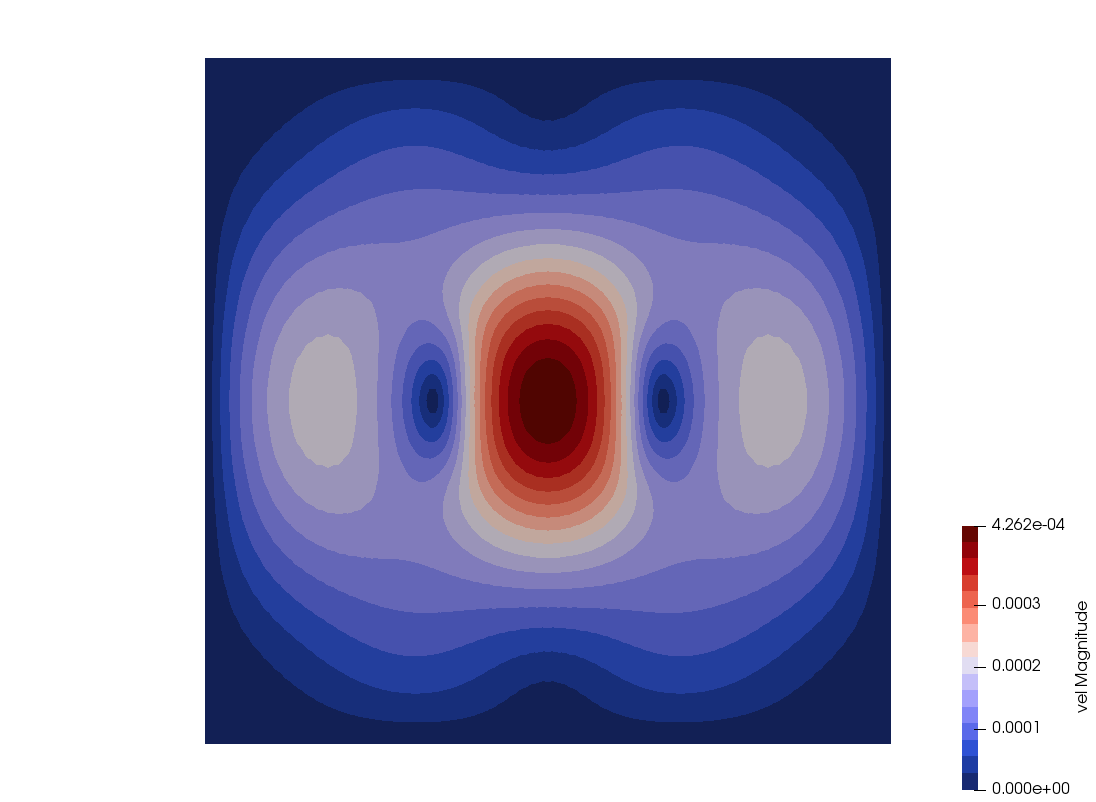
\includegraphics[width=3.84cm]{python_codes/fieldstone_78/results/block/vel_delta0p1}
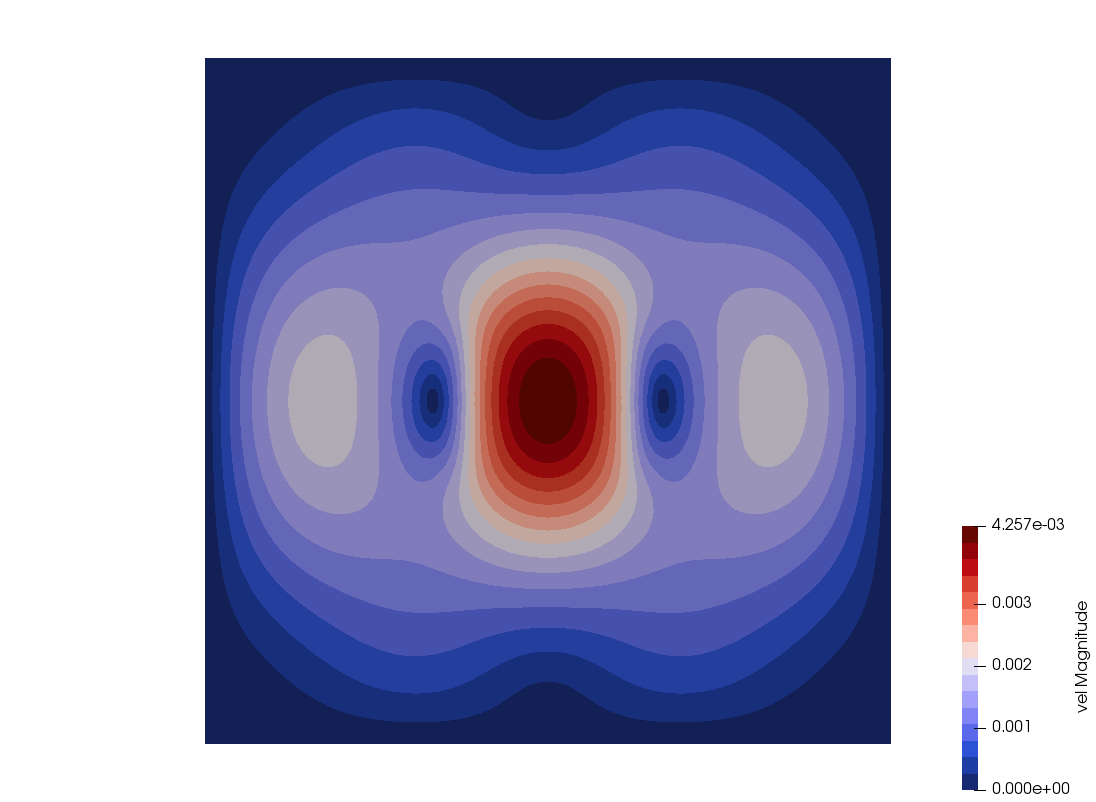
\includegraphics[width=3.84cm]{python_codes/fieldstone_78/results/block/vel_delta1}\\
{\captionfont Resolution 64x64. From left to right: $\delta=0.001,0.01,0.01,1$}
\end{center}

%..................................
\paragraph{Results - sinking block}

This is the same experiment as above, except for the geometry of the object 
which is now a sphere of radius 0.125.

\begin{center}
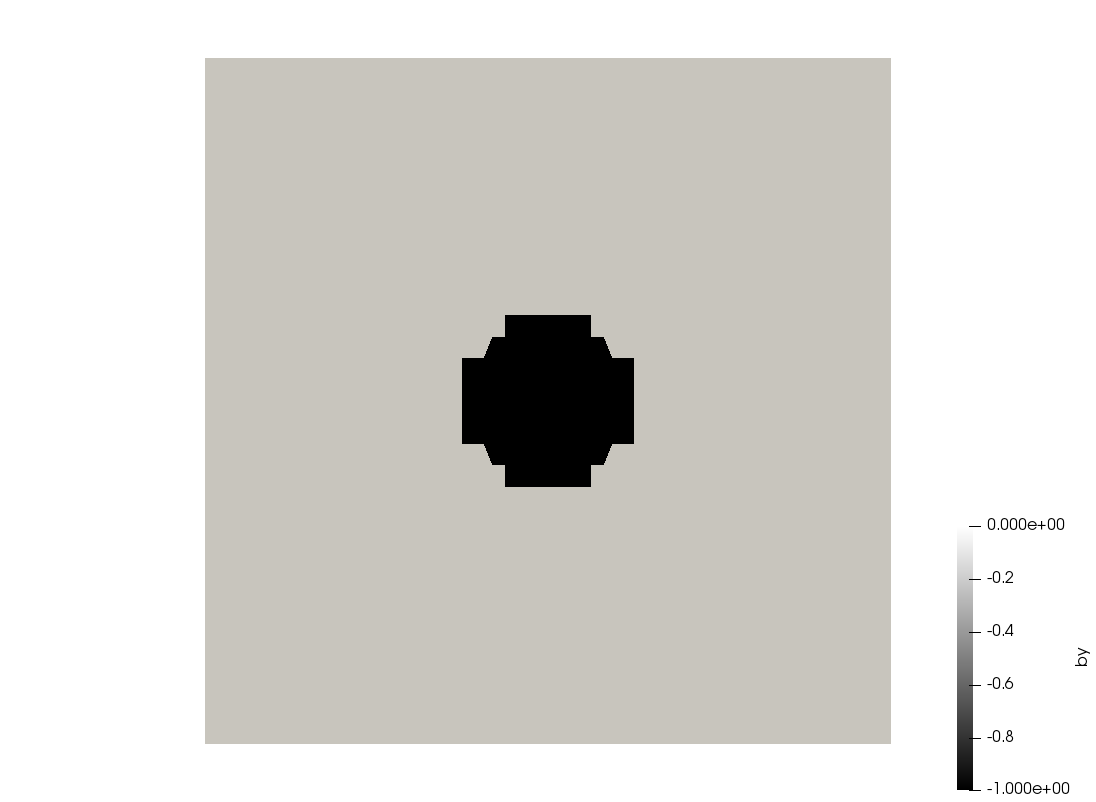
\includegraphics[width=3.84cm]{python_codes/fieldstone_78/results/sphere/by16}
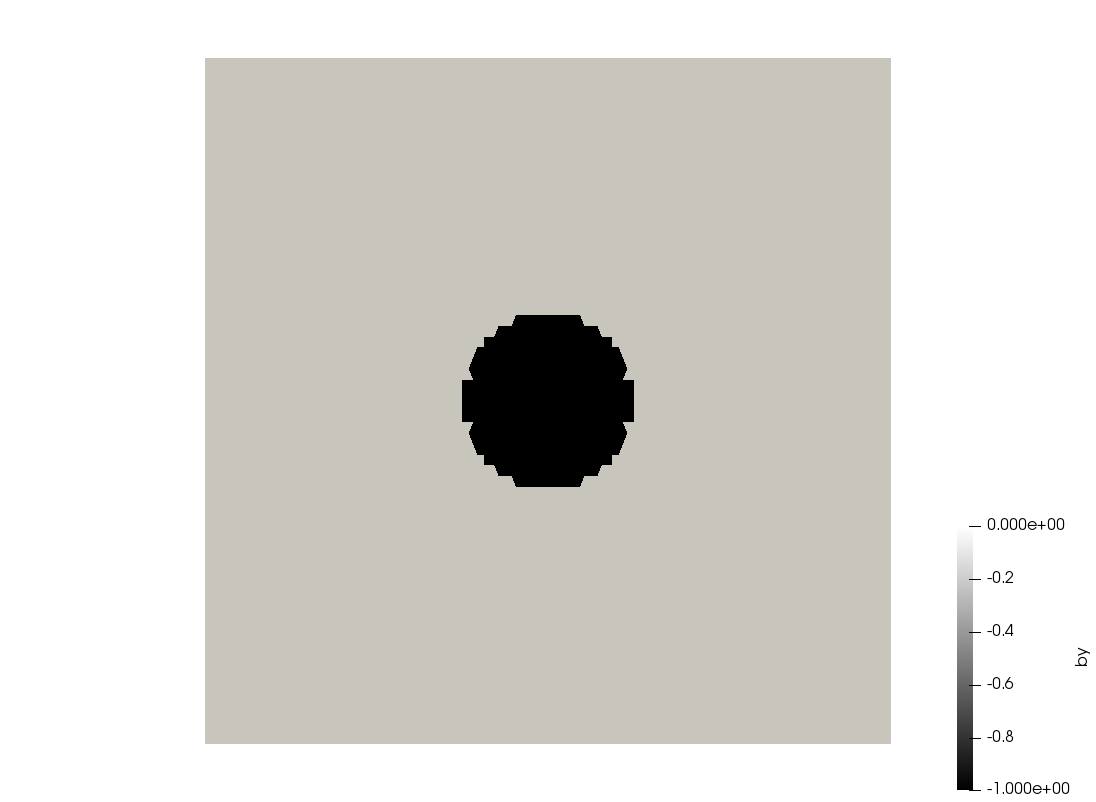
\includegraphics[width=3.84cm]{python_codes/fieldstone_78/results/sphere/by32}
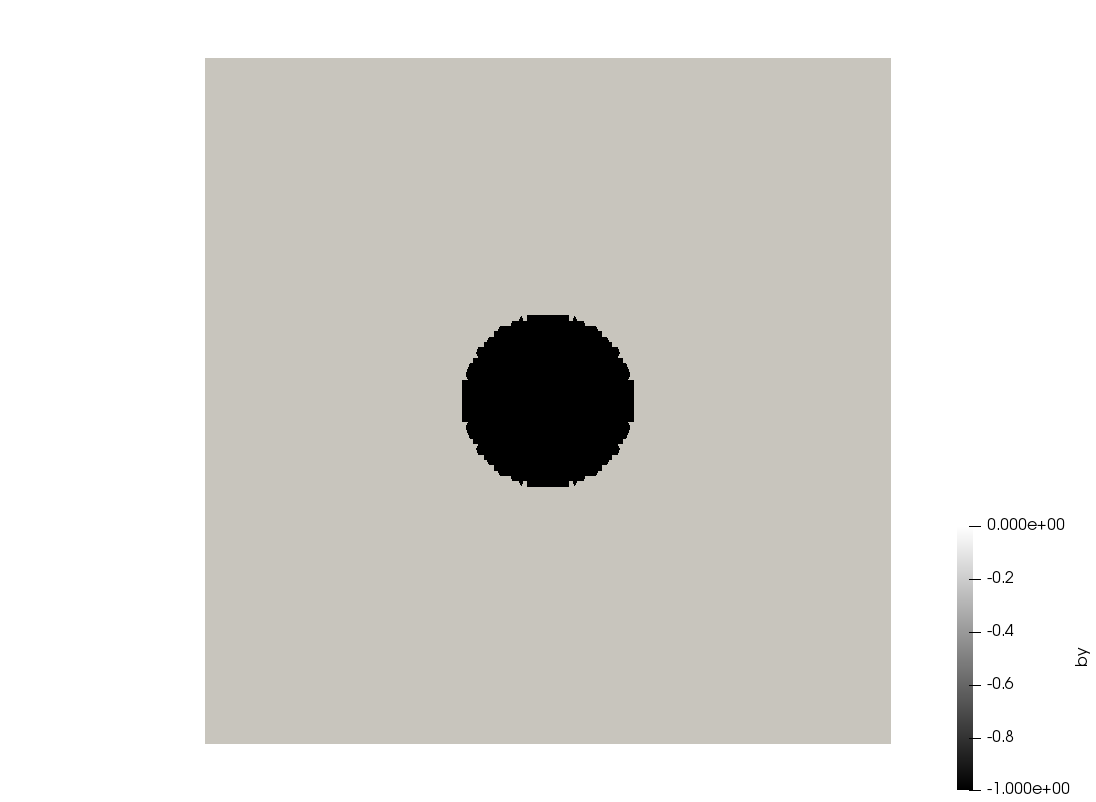
\includegraphics[width=3.84cm]{python_codes/fieldstone_78/results/sphere/by64}
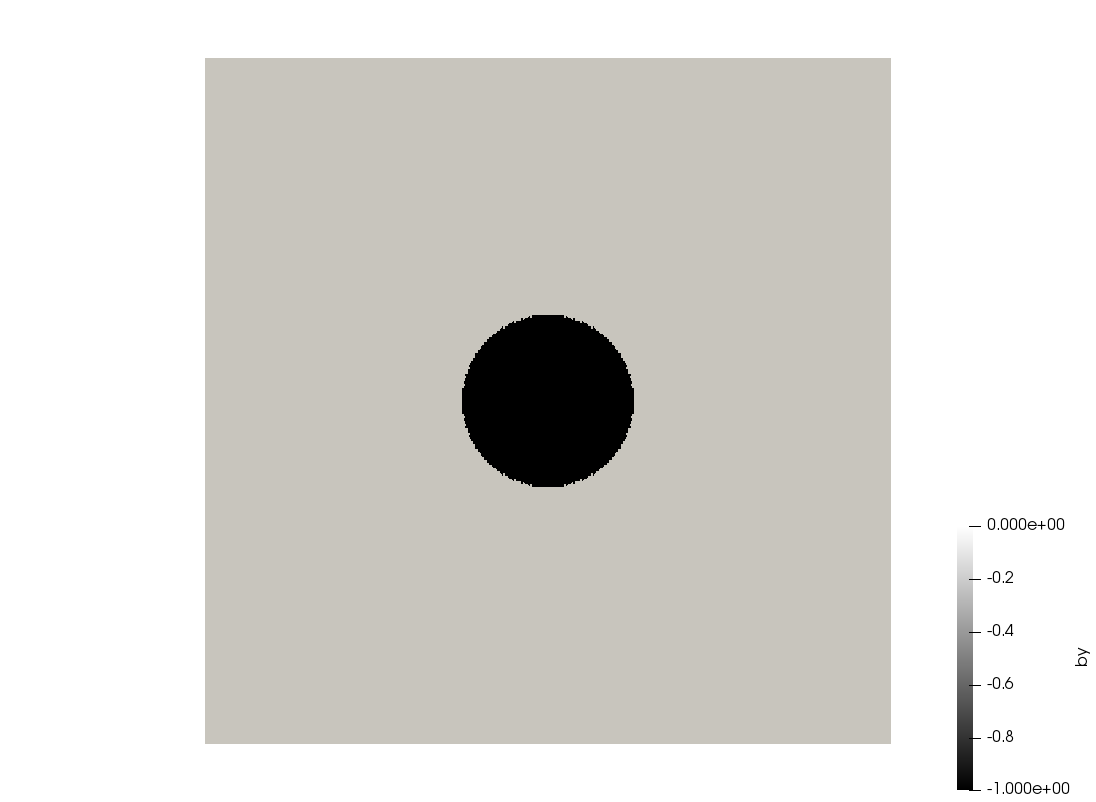
\includegraphics[width=3.84cm]{python_codes/fieldstone_78/results/sphere/by128}\\
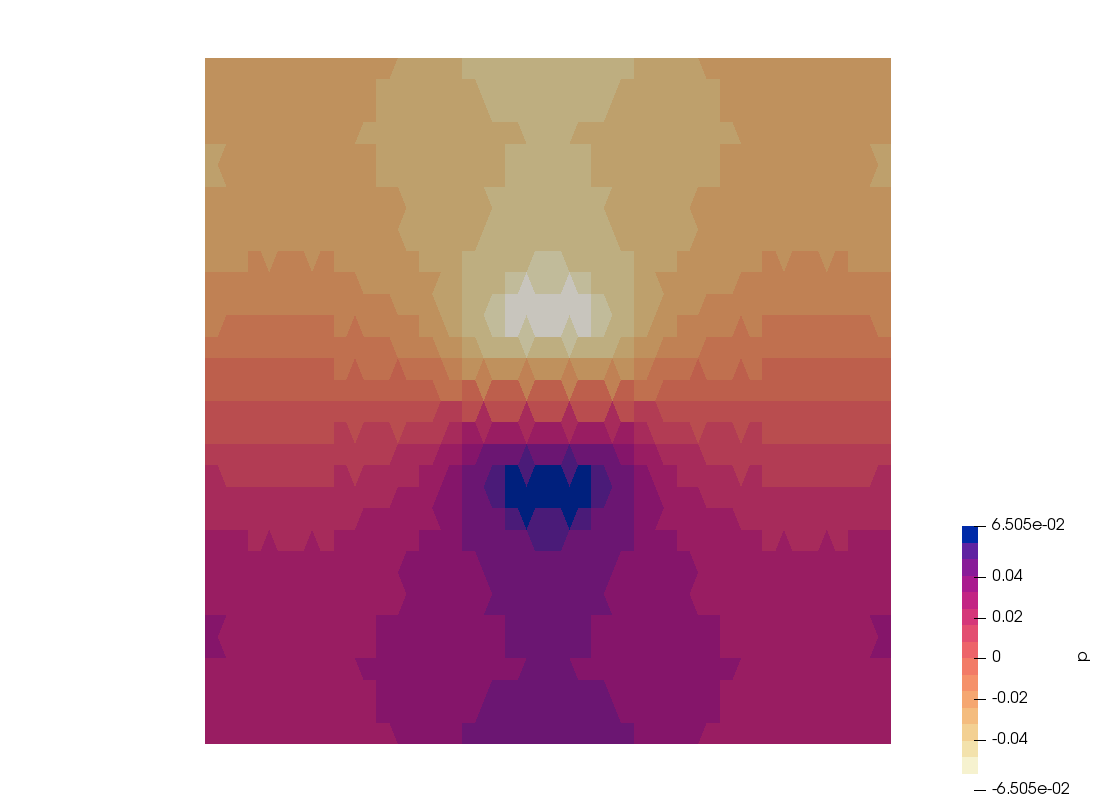
\includegraphics[width=3.84cm]{python_codes/fieldstone_78/results/sphere/p16}
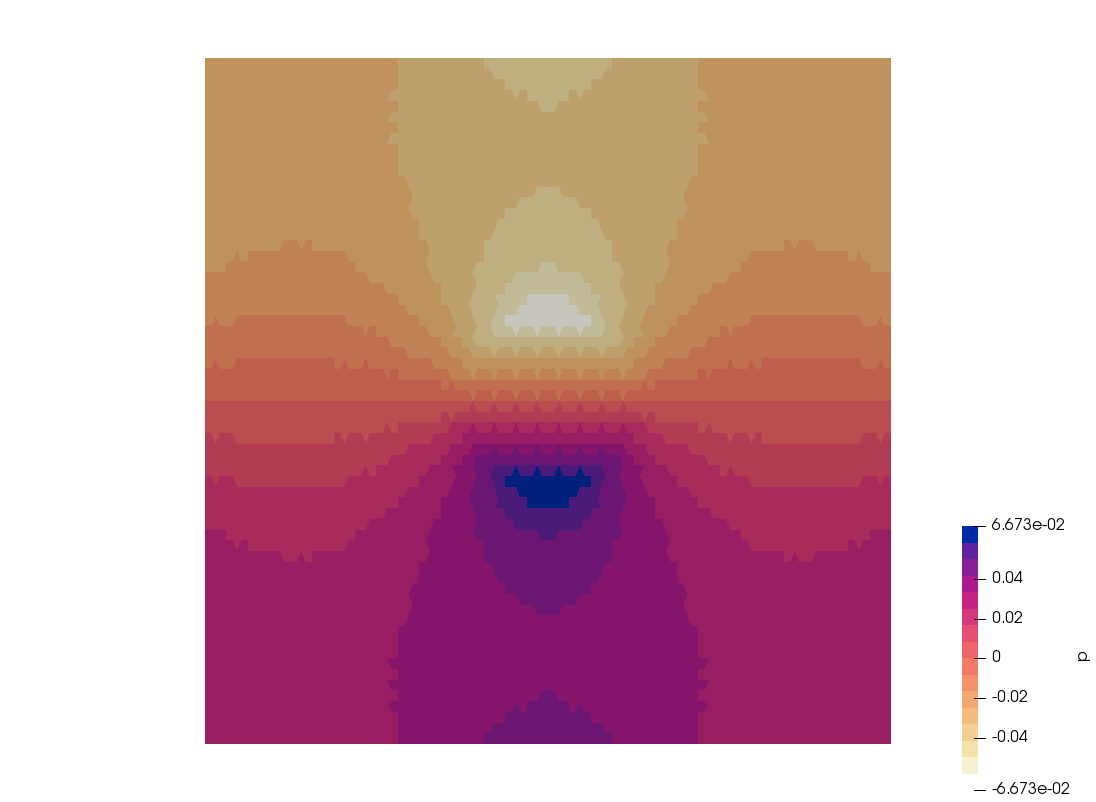
\includegraphics[width=3.84cm]{python_codes/fieldstone_78/results/sphere/p32}
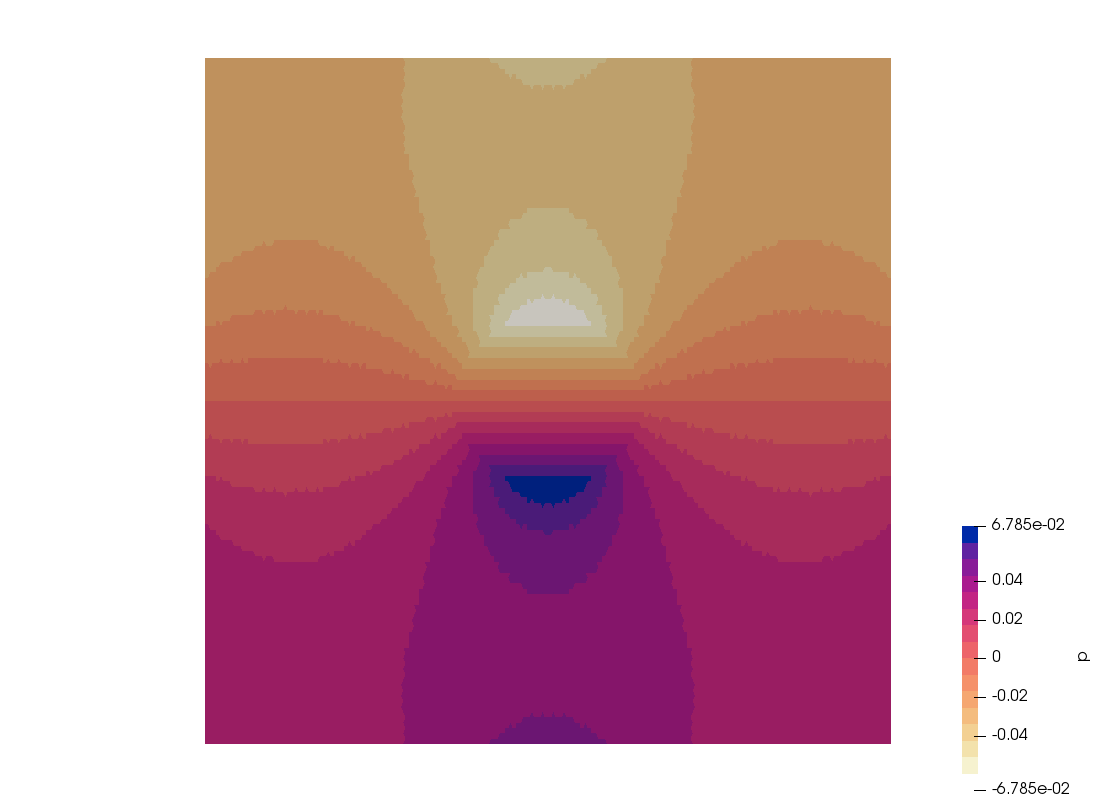
\includegraphics[width=3.84cm]{python_codes/fieldstone_78/results/sphere/p64}
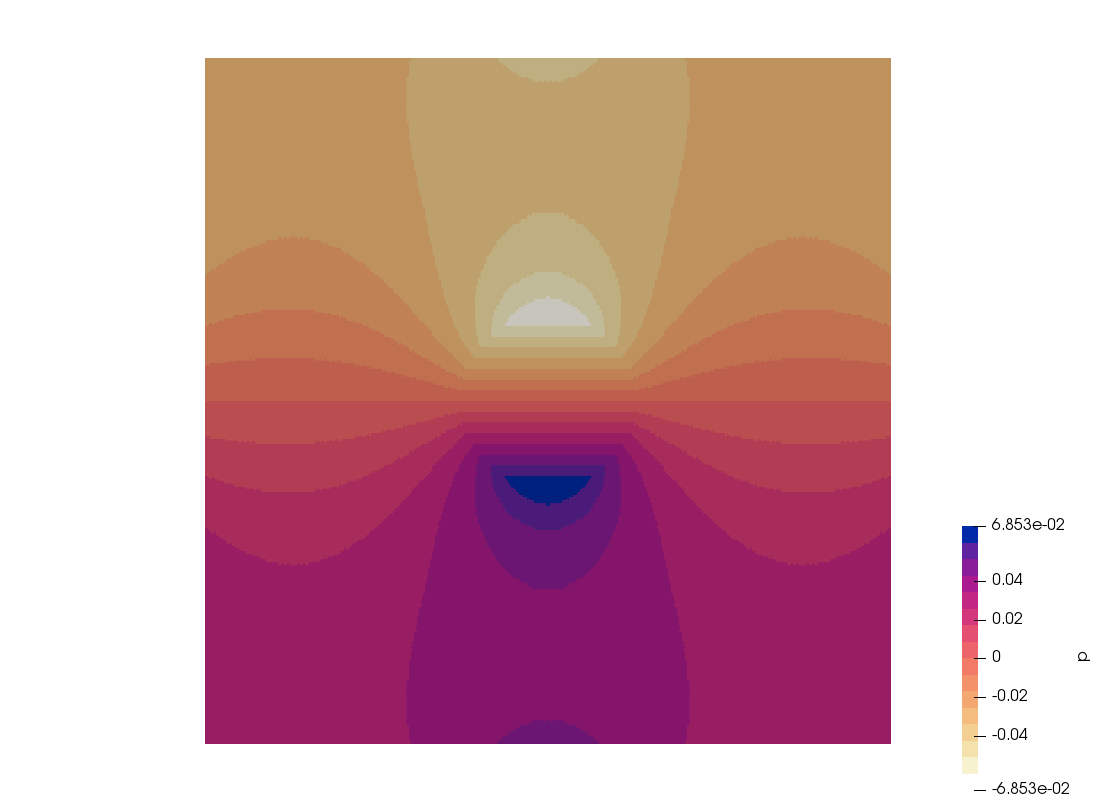
\includegraphics[width=3.84cm]{python_codes/fieldstone_78/results/sphere/p128}\\
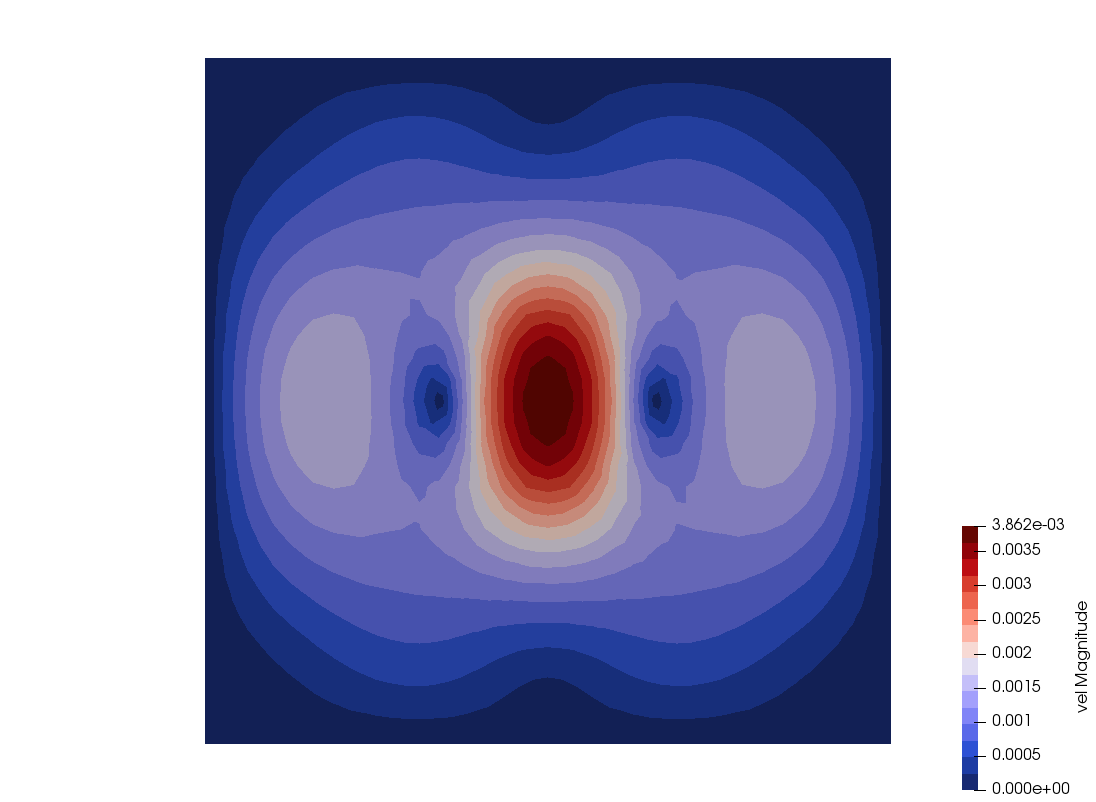
\includegraphics[width=3.84cm]{python_codes/fieldstone_78/results/sphere/vel16}
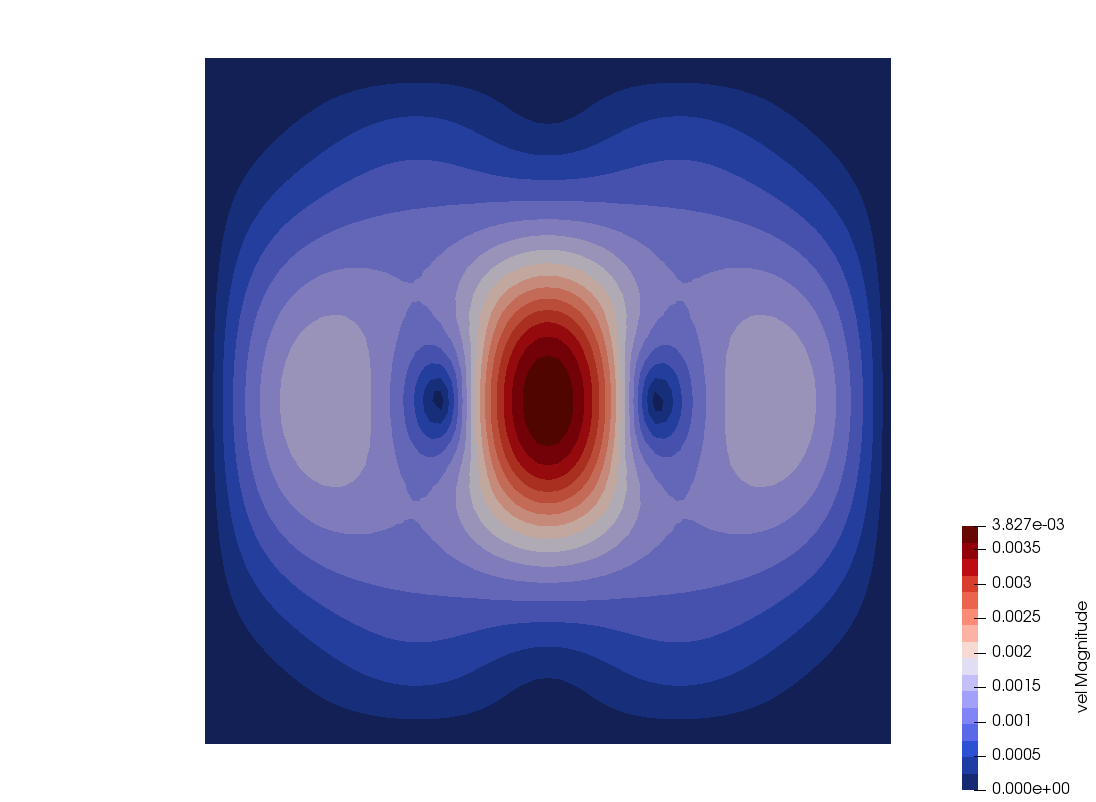
\includegraphics[width=3.84cm]{python_codes/fieldstone_78/results/sphere/vel32}
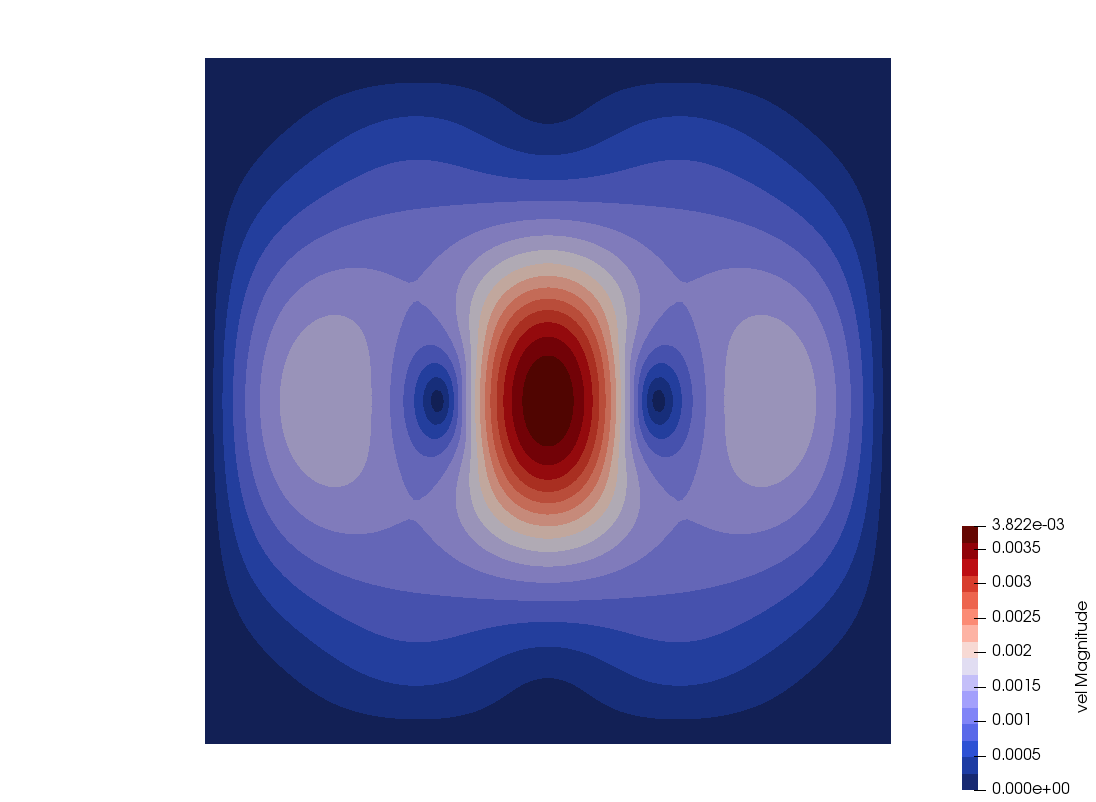
\includegraphics[width=3.84cm]{python_codes/fieldstone_78/results/sphere/vel64}
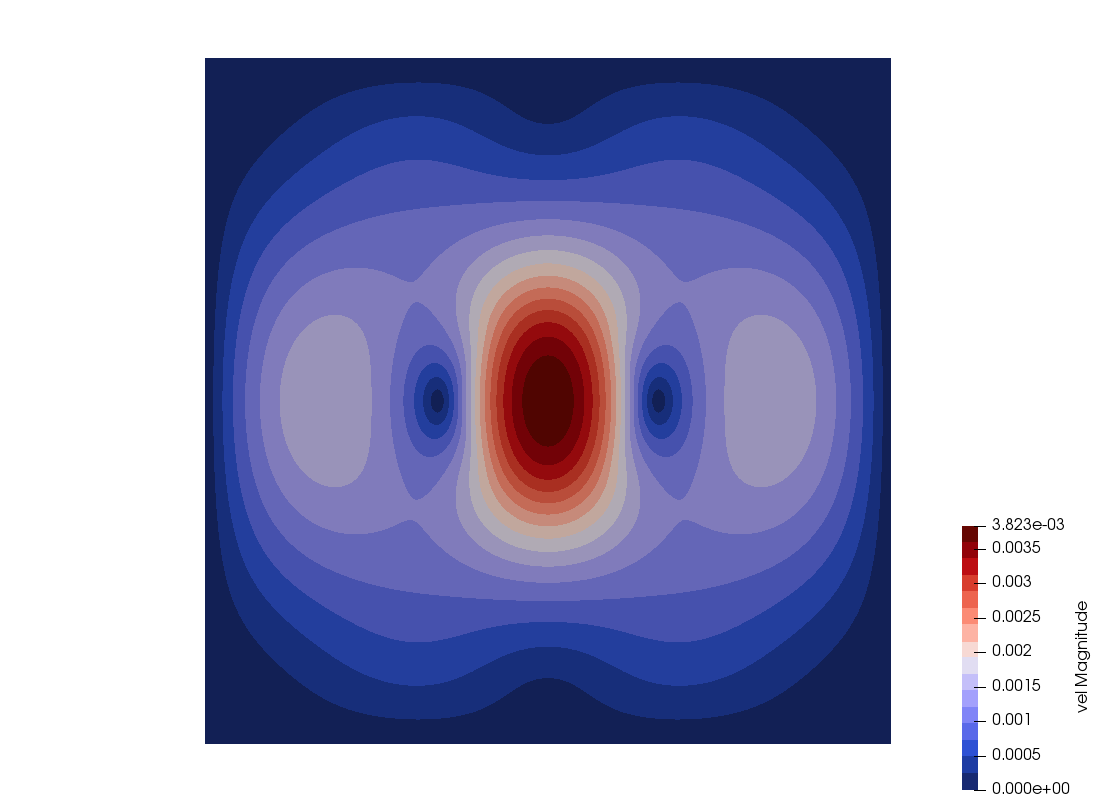
\includegraphics[width=3.84cm]{python_codes/fieldstone_78/results/sphere/vel128}\\
{\captionfont From left to right: 16x16, 32x32, 64x64, 128x128, $\delta=1$}
\end{center}


